%% LyX 2.3.6.1 created this file.  For more info, see http://www.lyx.org/.
%% Do not edit unless you really know what you are doing.
\documentclass[english]{vgtc}
\usepackage[T1]{fontenc}
\usepackage[latin9]{inputenc}
\usepackage{geometry}
\geometry{verbose,tmargin=1in,bmargin=1in,lmargin=1in,rmargin=1in}
\usepackage{graphicx}

\makeatletter
%%%%%%%%%%%%%%%%%%%%%%%%%%%%%% Textclass specific LaTeX commands.
\usepackage{mathptmx}
\usepackage{graphicx}
\usepackage{times}

%%%%%%%%%%%%%%%%%%%%%%%%%%%%%% User specified LaTeX commands.
%% Supported class options:

%\documentclass{vgtc}                          % final (conference style)
%\documentclass[review]{vgtc}                 % review
%\documentclass[widereview]{vgtc}             % wide-spaced review
%\documentclass[preprint]{vgtc}               % preprint
%\documentclass[electronic]{vgtc}             % electronic version

%% ``review'' and ``widereview'' are for review
%% submission, ``preprint'' is for pre-publication, and the final version
%% doesn't use a specific qualifier. Further, ``electronic'' includes
%% hyperreferences for more convenient online viewing.

%% Please use one of the ``review'' options in combination with the
%% assigned online id (see below) ONLY if your paper uses a double blind
%% review process. Some conferences, like IEEE Vis and InfoVis, have NOT
%% in the past.

%% Figures should be in CMYK or Grey scale format, otherwise, colour 
%% shifting may occur during the printing process.

%% We encourage the use of mathptmx for consistent usage of times font
%% throughout the proceedings. However, if you encounter conflicts
%% with other math-related packages, you may want to disable it.

%% If you are submitting a paper to a conference for review with a double
%% blind reviewing process, please replace the value ``0'' below with your
%% OnlineID. Otherwise, you may safely leave it at ``0''.
\onlineid{0}

%% declare the category of your paper, only shown in review mode
\vgtccategory{Research}

%% allow for this line if you want the electronic option to work properly
\vgtcinsertpkg

%% In preprint mode you may define your own headline.
%\preprinttext{To appear in an IEEE VGTC sponsored conference.}


%% This is how authors are specified in the conference style

%% Author and Affiliation (single author).
\author{Brendan Robert\thanks{e-mail: bdvision@colostate.edu}}

\makeatother

\usepackage{babel}

\CCScatlist{
  \CCScatTwelve{Human-centered computing}{Keyboards}{}{};
  \CCScatTwelve{Human-centered computing}{Touch screens}{}{}
}

\abstract{Touchscreen-based computers allow rapid experimentation with novel
keyboard layouts compared to physical keyboards. The goal of this
experiment is to compare a traditional QWERTY keyboard layout with
a newer optimized keyboard layout based on a Metropolis algorihm to
see how users perform differently, and also if adding hints helps
users acclimate to the different keyboards any better.}

\begin{document}
\title{Badvision Keyboard}
\maketitle

\section{Introduction}

Touchscreen users are reported to have much more discomfort and fatigue
with touchscreen keyboards \cite{chaparro13} compared to traditional
physical analogues. However, there are environments where touchscreens
are the most appropriate form factor and therefore there is a need
to aid touchscreen users to reduce errors and improve overall efficiency
where possible. Overall this can lead to an improved touchscreen user
experience. Aside from commercial settings where tablets are frequently
used such as industrial and medical, users with poor vision or who
are inexperienced (children) can benefit from visual typing aids as
these classes of users are more likely to look at the keyboard while
typing. \cite{alhabri19} This keyboard would work in place of any
standard soft keyboard overlay. The difference is whereas some keyboards
today offer suggested words above the keyboard overlay, the Metropolis-based
\textquotedblleft Badvision\textquotedblright{} keyboard will highlight
suggested keys for the user to press next. This applies to general
keyboard input but in this limited application the subject domain
will be focused on natural common English phrases. The predictive
text model will not account for technical or scientific words, nor
will it be trained on patterns of text found in programming languages.
This is described more in the Trials section below. This soft keyboard
would be ideally suited for any kind of on-screen overlay input scenario
on a touchscreen such as an iPad or a Surface laptop. However, there
is potential to optimize for smaller screen sizes but that will not
be considered as part of this study.

\section{Background}

Predictive keyboard features, aka Predictive Text Generation was researched
as early as 1988 by John Darragh \cite{darragh88}. His PhD dissertation
proposes an early model for auto-correction named \textquotedblleft The
Reactive Keyboard\textquotedblright{} (shown in figure 1) which to
a good degree also serves a fair empirical study of the area of predictive
text dating back even further to early work by Dennis Ritchie and
Ken Thompson in the form of the UNIX Predict keyboard utility. The
Reactive Keyboard thesis goes into great length to examine various
implementation choices for modeling a search algorithm for predictions
as well, though modern readers are not as confronted with tradeoffs
to achieve efficiency and responsiveness on modern hardware. With
Witten and James, Darragh continued this work further \cite{darragh90}
to take the Reactive Keyboard to implementation on the Macintosh platform.
The implementation of this is more of a smart text editor application
which provides auto-correction suggestions as the user is typing.
The state of the art at the time required users to ask programs to
scan documents for spelling errors, so having a quick and efficient
auto-suggestion feature was at the time a very novel concept, but
in a practical sense the authors note that users with disabilities
such as cerebral palsy reported they felt predictive typing aids were
strongly beneficial. It is worthy of mention this effect is a major
consideration and inspiration to continue examining input methods
to help the disabled! 

\begin{figure}[htbp]
\begin{centering}
\textsf{\includegraphics[scale=0.45]{\string"reactive keyboard\string".png}}
\par\end{centering}
\caption{The Reactive Keyboard}
\end{figure}

Alhabri et. al propose a tablet keyboard solution named \textquotedblleft WiseType\textquotedblright{}
\cite{alhabri19} which \textquotedblleft combines different visual
representations for grammar and spelling errors, accepted predictions,
and auto-corrections.\textquotedblright{} WiseType (figure 2) provides
a smart delete key which allows the user to go back to the start of
their first mistake, however on-screen feedback is limited to the
area of text entry itself. The keyboard overlay shown offers no visual
feedback on its own except for suggested words that appear over the
keys, like modern keyboard overlays on modern smart phones. Also like
some modern touchscreen keyboards, WiseType also auto-corrects words
in some cases.

\begin{figure}
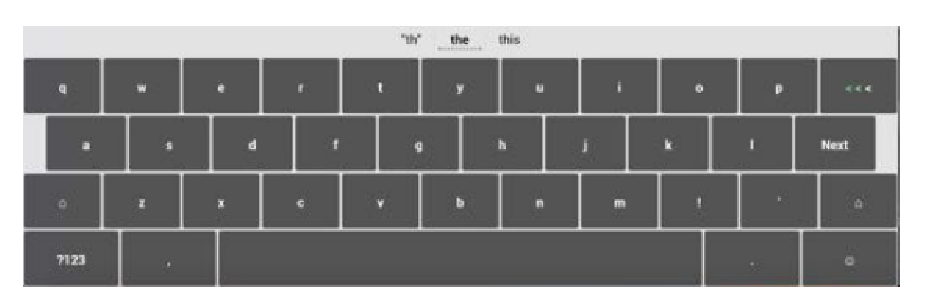
\includegraphics[scale=0.5]{WiseType}

\caption{WiseType Keyboard}
\end{figure}

Sono and Hasegawa \cite{Sono19} propose projection mapping (figure
3) onto a physical keyboard as an instructional aid to teach typing.
In the case of this typing tutor approach, the next key expected is
known absolutely and therefore only one key needs to be highlighted
at a time for the user. Their results were reported quantitively in
speed and error, also time to press the first key was measured as
well. They also provided survey results to gauge how confident users
felt about their typing before and after. 

\begin{figure}
\includegraphics[scale=0.6]{\string"Overlay Projection\string".png}

\caption{Sono/Hasegawa Overlay Projection}
\end{figure}

In designing the ideal onscreen keyboard, it became necessary to find
what conclusions have already been reached regarding ideal layouts.
The primary independent variable is to measure user performance against
the presence or absence of typing suggestions, and so the keyboard
layout should also allow greater chance of success. Zhai, Hunter and
Smith designed a keyboard layout (figure 4) quantitatively using a
Metropolis random walk algorithm to produce a layout capable of 43.1
WPM performance. \cite{Zhai00}

\begin{figure}
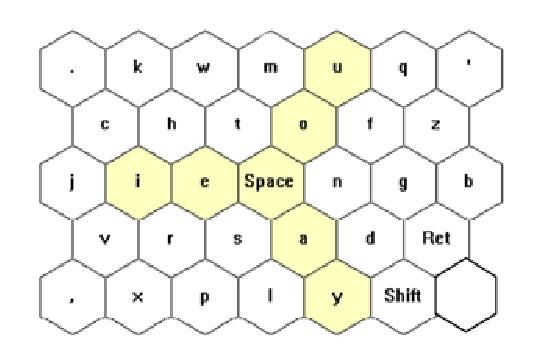
\includegraphics[scale=0.9]{Metropolis}

\caption{Metropolis Keyboard (unweighted layout)}
\end{figure}

Though promising, this was further improved by Zhai and Smith one
year later \cite{Zhai01} by weighting the alphabetical ordering of
the letters, helping novice users locate keys more quickly, up to
9\% improvement over the previous Metropolis keyboard. The weighted
layout, shown in figure 5, is the layout which will be used in the
experiment alongside a traditional QWERTY layout.

\begin{figure}
\includegraphics[scale=0.16]{\string"metropolis keyboard weighted\string".png}

\caption{Metropolis Keyboard weights biased on alphabetical ordering}
\end{figure}


\section{Methodology}

\subsection{Subject Selection}

The subject pool available for this experiment is a geographically
distributed convenience sample. I will attempt to make this experiment
available over the internet so that other people can volunteer if
they have an iPad or a Surface Book. Similar studies have roughly
a half dozen subjects, with trials taking as long as 45 minutes. To
avoid environmental issues (see section on extraneous and confounding
variables) the trial duration should be reduced to 10-15 minutes,
thus reducing probability of distraction during the test. Also, longer
tests complicate locating willing volunteers so this solves two problems.
With the number of samples per subjects reduced, a data set comparable
to similar studies can be obtained by increasing the desired subject
pool to approximately 20 subjects.

\subsection{Software Test Apparatus}

The software test apparatus will be provided as a website. The user
will be identified with a cookie in case they leave and come back,
or in case they choose to try again later. When they first arrive,
they will be presented with a small page of instructions explaining
the test. After then they will provide optional details about themselves
such their age range, and if they have any physical conditions, injuries
that affect their ability to use computers normally. After this they
will be provided a set of text shown at the top of the screen and
will be asked to type what they read on the screen. As they type their
response will be shown below the provided text. Incorrect letters
will appear but will be replaced with correct letters as they continue
typing. If they omit one letter and type 2 letters that proceed it,
then it will show that letter in red and continue showing their typed
response. The goal is to have the keyboard auto-correct the user so
that they can stay focused on pressing the next keys in sequence otherwise
measuring typing performance and accounting for user corrections adds
more noise to the data. This auto-correct behavior will remain consistent
for all trials. Explored further in the later section on confounding
variables, it is important to ensure the physical size of the keyboard
layout is consistent for all participants. A Logitech K830 keyboard
will be used for comparison, which has keys laid out in a 26cm x 10cm
arrangement due to its compact but usable format. A Microsoft surface
14\textquotedblright{} laptop has physical view area dimensions larger
than that (28.5cm x 18.5cm), and an iPad Pro has (30.5cm x 22cm).
If there is no way to automatically adjust to the individual display,
the apparatus will need a calibration step added to ensure the size
is correct. For example, having the user place a common object such
as a credit card on the screen and sliding controls to conform to
that shape could quickly identify pixel size vs screen size ratios
appropriate to that specific device. 

\subsection{Trials}

The trials will test the same typing test against two independent
variables, Layout and Presence of highlighted key suggestions, each
having two levels. The variations are captured in 4 trials, which
will be presented to the participant in an order determined by a pre-selected
random sequence that will be assigned to each visitor (4x4 Latin square).
Ultimately the ideal apparatus being tested is in Trial D, and the
other trials will seek to identify if the independent variables in
that apparatus have any statistical significance in the data observed.
Trial A: QWERTY style keyboard layout, with no typing suggestions
offered. Trial B: QWERTY style keyboard layout, with typing suggestions
offered. Trial C: \textquotedblleft Zhai/Smith\textquotedblright{}
Metropolis style keyboard layout, with no typing suggestions offered.
Trial D: \textquotedblleft Badvision\textquotedblright{} Metropolis
style keyboard layout, with typing suggestions offered. For trials
B and D, the typing suggestions are offered by highlighting the three
or four most likely keys the user will press next, based on a simple
Markov-chain predictor trained against the sample set of keystroke
combinations. The goal is to have predictive-like capabilities that
mimic real-world behavior and ensure that one suggestion offered will
always be the correct response. The response of the predictor is a
major factor, it only has to be guaranteed to offer correct predictions
for the typing samples provided so that the user key selection is
reduced to matching from provided samples and the suggestions are
better-than-random, so they are not distracting. There are some key
sequences which will have fewer suggestions and might offer only one
option, such as if the user types \textquotedblleft ZEA\textquotedblright{}
then the only likely next choice is \textquotedblleft L\textquotedblright .
However, the next sequence considered will have more suggestions because
\textquotedblleft EAL\textquotedblright{} might be followed by \textquotedblleft E\textquotedblright{}
or \textquotedblleft A\textquotedblright{} depending on if the user
were typing \textquotedblleft ZEALAND\textquotedblright{} or \textquotedblleft SEALED.\textquotedblright{} 

\subsection{Counfounding and Extraneous Variables}

There are many extraneous variables that cannot be measured or controlled
for this experiment but where possible we can attempt to identify
these and understand their possible effects. Firstly, the subject
pool is a convenience selection, which limits the generalization potential
of the collected data to a wider population. Therefore, in providing
analysis of the results it is important to appropriately frame the
context of the application of this data. Secondly, the subjects will
choose their environment and time for participating in the experiment
and that precludes the ability to offer a distraction-free environment.
The best that can be afforded is a careful wording of the instructions
to ensure the participant is in a quiet distraction-free setting for
the duration of the tests. Also, the user will press a button to begin
each trial when they are ready, so this can help them balance the
distractions of their environment between trials. As mentioned earlier,
the test will be designed to take a duration of 10-15 minutes which
is shorted compared to other similar studies, but that can reduce
the probability of environmental distraction from interfering with
the data. Other than measuring how long they spend on the instruction
pages, there is no reasonable way to measure or control the individual
participants\textquoteright{} environments but hopefully the mitigation
strategies will help. The confounding variable that affects this experiment
most directly is the level of expertise of the user, specifically
their learned typing proficiency. It is expected that an experience
typist would quickly adapt to the touchscreen and touch-type. Such
users would certainly show little or no improvement with the suggested
keys lighting up, because they would not be looking at the keyboard
in the first place. We can control this confounding variable to test
the primary independent variable by introducing the second independent
variable of the keyboard layout. This puts the experienced QWERTY
typists on the same level as less-experienced \textquotedblleft hunt-and-peck\textquotedblright{}
typists. Another confounding variable that could affect user performance
is that each user will use their own device which could be any physical
size. Because of the variety of product dimensions, careful design
will need to be exercised to ensure the physical size of the soft
controls is the same across devices ahead of time, and the device
used by each participant as well as any detectable settings such as
zoom level should be recorded with the user survey data in case their
device was not accounted for in the apparatus design. Users will be
requested to use a tablet-sized device to ensure that in landscape
mode it is capable of a near-full dimension of a physical QWERTY keyboard. 

\subsection{Data Collection}

At the beginning of the experiment, a brief survey will be offered
to capture general demographics: 
\begin{itemize}
\item Participant age (provided as ordinal scale of age groups: 5-10, 10-15,
15-20, etc.) 
\item Participant device details (brand/model, open-ended) 
\item Browser user agent string (system-provided) 
\item Where is device relative to user? (In lap, on tabletop, on a stand,
Closed selection)
\item Time and date as well as local user\textquoteright s time zone (system-provided)
\item Physical conditions that impair normal computer use (fatigue, past/present
injuries, visual acuity affects, vertigo, cerebral palsy Closed selection
of options with an \textquotedblleft Other\textquotedblright{} box) 
\item Degree to which they feel it impacts their normal computer use (1-7
scale)
\end{itemize}
For each key stroke in each of the trials, the following will be stored: 
\begin{itemize}
\item Prompt the user is expected to type 
\item Time in milliseconds since the start of the trial when key down was
detected 
\item Time in milliseconds since the start of the trial until key up 
\item The key expected 
\item The key entered (if SKIP that means we detected a skipped key) 
\item If the keystroke was correct (1) or an error (0) 
\item X and Y coordinates of where the user pressed (relative to the upper-left
of the keyboard control) -- this should be measured in precise physical
units, or at least recorded with calibration data so that cross-device
data comparison is possible. 
\end{itemize}
After raw collection is completed for a trial, the information is
then converted into more general information: - Speed, measured in
words per minute. This is measured as correct keys per second / 5
- \% of key strokes which were errors Both the summary data and the
raw data will be retained in case there are additional insights of
the data that could become useful. One possible area of exploration
is to measure error not by incorrect keystrokes but by the distance
between the detected key and the expected key. \cite{Jain11} This
would allow less of a penalty for keystrokes that were \textquotedblleft fat
finger\textquotedblright{} entries of neighboring keys. 

\section{Demonstration}

This project will be demonstrated with a live website demo for audience
members to explore on their own, and a recorded presentation explaining
the project and its findings with a demo component showing a recording
of the presenter using the website and viewing the captured data.

\section{Expected Outcome}

It would be ideal if the Trial C (keyboard with no suggestions) lives
up to the promise of the research of Zhai and Smith. With predictive
highlighting it is also hoped that users will have an easier time
learning the new keyboard layout (Trial D) and using it with fewer
errors, if not benefitting from an improved typing speed. Other research
on adaptive predictive text keyboards offers promise not just for
novice users but also people with physical disabilities. This project
is not specifically studying the effects of this technology on that
part of the population but having additional options for folks with
disabilities can only be a net positive result.

\bibliographystyle{abbrv}
\bibliography{proposal}

\end{document}
